\documentclass{article}
\usepackage[margin=1in]{geometry}
\usepackage{amsmath,amsthm,amssymb}
\usepackage{bbm,enumerate,mathtools}
\usepackage{tikz,pgfplots}
\usepackage{chessboard}
\usepackage[hidelinks]{hyperref}
\usepackage{multicol} % Problem 35

\newenvironment{question}{\begin{trivlist}\item[\textbf{Question.}]}{\end{trivlist}}
\newenvironment{note}{\begin{trivlist}\item[\textbf{Note.}]}{\end{trivlist}}
\newenvironment{references}{\begin{trivlist}\item[\textbf{References.}]}{\end{trivlist}}
\newenvironment{related}{\begin{trivlist}\item[\textbf{Related.}]\end{trivlist}\begin{enumerate}}{\end{enumerate}}


\begin{document}
\rating{2}{3}
Polysticks can be used to model nets of a
(not necessarily convex) polyhedron with square faces, by thinking of the
vertices of the polystick as faces of a polycube and the edges of the polystick
as Scotch tape connecting two faces at an edge.
\begin{figure}[ht!]
  \centering
  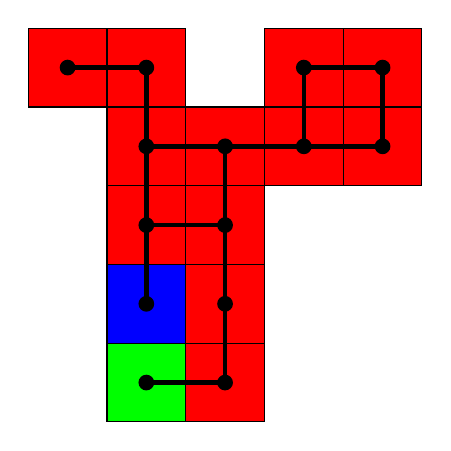
\begin{tikzpicture}[scale=1.0]
    \foreach \x/\y/\c in {
      -1/4/red, 0/4/red,            2/4/red, 3/4/red,
                0/3/red,   1/3/red, 2/3/red, 3/3/red,
                0/2/red,   1/2/red,
                0/1/blue,  1/1/red,
                0/0/green, 1/0/red} {
      \draw[fill=\c] (\x - 1/2,\y - 1/2) rectangle (\x + 1/2, \y + 1/2);
      \fill (\x,\y) circle (0.1);
    }
    \draw[ultra thick]
      (-1,4)--(0,4)--(0,3)--(1,3)--(2,3)--(3,3)--(3,4)--(2,4)--(2,3)
      (0,3)--(0,2)--(1,2)--(1,3)
      (1,2)--(1,1)--(1,0)--(0,0)
      (0,2)--(0,1);
  \end{tikzpicture}
  \hspace{1cm}
  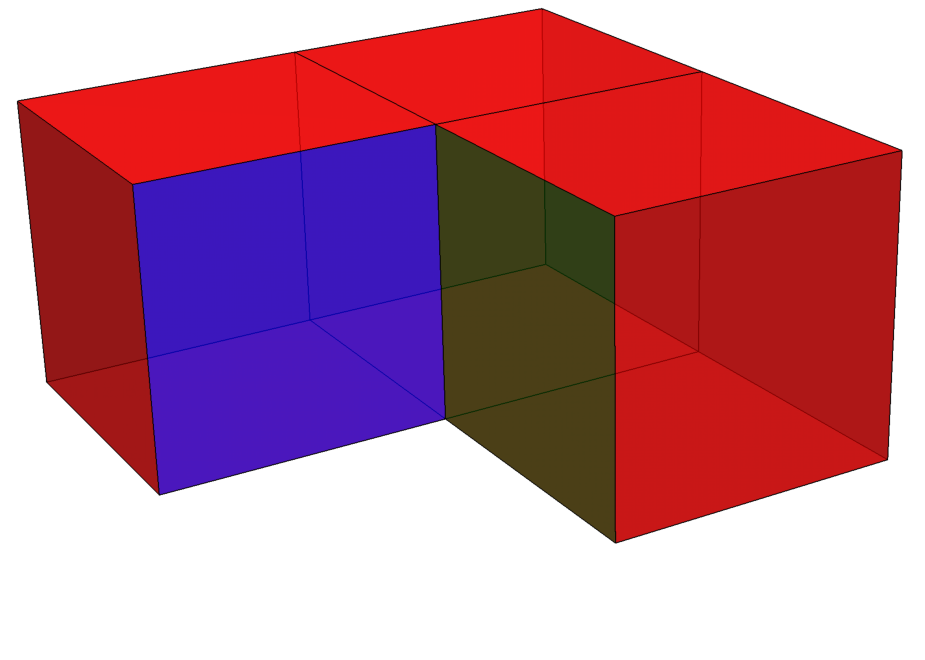
\includegraphics[scale=0.6]{assets/123_problem/polyhedron_unboxed}
  \caption{
    A polystick with 15 edges that models a net of a polycube.
  }
\end{figure}

\begin{question}
  Which polysticks can be used to realize a polyhedron with square faces?
\end{question}

\begin{related}
  \item Is there a computationally efficient algorithm of determining whether
    a given polystick can be folded into a polyhedron?
  \item Is there a computationally efficient algorithm of determining the number
    of ways a given polystick can be folded into a polyhedron?
  \item How many polysticks can be folded into a rigid structure with no degrees
    of freedom?
  \item What if we model polyhedra with triangular faces instead? Pentagonal?
\end{related}

\begin{references}
  \item \url{https://en.wikipedia.org/wiki/Polystick}
\end{references}
\end{document}

% vertices:={
% {0,0,0},(*1*)
% {0,1,0},(*2*)
% {1,0,0},(*3*)
% {1,1,0},(*4*)
% {0,0,1},(*5*)
% {0,1,1},(*6*)
% {0,2,1},(*7*)
% {0,2,0},(*8*)
% {1,0,1},(*9*)
% {2,0,1},(*10*)
% {2,0,0},(*11*)
% {1,1,1},(*12*)
% {2,1,1},(*13*)
% {2,1,0},(*14*)
% {1,2,0},(*15*)
% {1,2,1}(*16*)
% }
% faces:={
% {1,2,4,3},{1,2,6,5},{7,8,2,6},{1,3,9,5},{3,9,10,11},{5,6,12,9},{12,13,10,9},{4,14,11,3},{13,10,11,14},{16,15,8,7},{16,12,6,7},{15,4,2,8}
% }
% Graphics3D[
% {Opacity[0.7],
% Red,
% Polyhedron[vertices,faces],
% Blue,
% Polyhedron[vertices,{13,14,4,12}],
% Green,
% Polyhedron[vertices,{12,4,15,16}]
% },
% Boxed -> False
% ]
